\addtocontents{toc}{\protect\booltrue{specialtoc}}

\chapter{Bit Error Rate (BER) for BPSK Modulation} \label{appendA}
\pretocmd{\chapter}{\addtocontents{toc}{\addvspace{-14pt}}}{}{}
\addcontentsline{toc}{chapter}{APPENDIX A: Bit Error Rate (BER) for BPSK Modulation}

\begin{figure}[!h]
%\captionsetup{list=no}
%\stepcounter{figure}
\centering
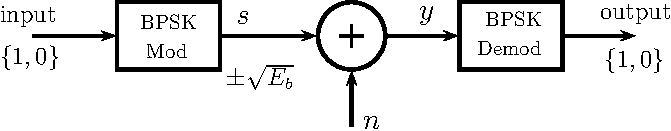
\includegraphics[width=\textwidth]{./append1/BPSK_txrx}
%\NLofcaption{BPSK transmitter and receiver}
%\legend{\figurename~\thefigure: BPSK transmitter and receiver.
\caption{BPSK transmitter and receiver.}
\label{figI:BPSK_txrx}
\end{figure}
\noindent In Binary phase shift keying scheme, the input bits 1 and 0 could be represented by two analogue levels; $ \sqrt{E_b} $ for symbol 1 and $ -\sqrt{E_b} $ for symbol 0. Figure~\ref{figI:BPSK_txrx} shows a block diagram for a typical BPSK transmitter and receiver. 

\par When the signal is to be sent over the channel it will experience noise $ n $, which is additive white Gaussian noise.




The received signal:
 \[
	{y}=
	\begin{cases}
	s_1+n, &\text{ if bit 1 is transmitted} \\
	s_0+n, & \text{if bit 0 is transmitted} 
	\end{cases} 
	\]
	The conditional probability distribution function (PDF) (Figure~\ref{figI:BPSK_BER}) of $ y $ for the two signals are:
	\begin{align}
	f(y/s_0)&=\dfrac{1}{\sqrt{\pi N_0}}e^{\frac{{-(y+\sqrt{E_b})}^2}{N_0}}\\
	f(y/s_1)&=\dfrac{1}{\sqrt{\pi N_0}}e^{\frac{{-(y-\sqrt{E_b})}^2}{N_0}}
	\end{align}
	
	\begin{figure}[htb]
	\captionsetup{list=no}
	%\stepcounter{figure}
	\centering
	\def\svgwidth{\textwidth} % Defining the width since Inkscape hasn't done this yet in the .pdf_tex file
	%\small
	\input{./append1/BPSK_BER.pdf_tex}
	%\caption[]{The conditional probability distribution function with BPSK}
	%\legend{\figurename~\thefigure: The conditional probability distribution function with BPSK.}
	\caption{The conditional probability distribution function with BPSK.}
	\label{figI:BPSK_BER}
	\end{figure}
	
Assuming an equiprobable transmitted bits, i.e, $ P(s_1)=P(s_0)=\dfrac{1}{2} $, the threshold $ 0 $ is the optimal decision boundary.
if the received signal is greater than the threshold, the receiver decides $ s_1 $ was transmitted, otherwise, it decides that $ s_0 $ is transmitted. mathematically;
\begin{align*}
y&>0 \Rightarrow s_1\\
y&\leq 0 \Rightarrow s_0
\end{align*}
The probability of error given $ s_1 $ was transmitted:
\begin{align}
f(e|s_1)&=\dfrac{1}{\sqrt{\pi N_0}}\int\limits_{-\infty}^{0}e^{\frac{{-(y-\sqrt{E_b})}^2}{N_0}}dy\\
&=\dfrac{1}{\sqrt{\pi}}\int\limits_{\sqrt{\frac{E_b}{N_0}}}^{\infty}e^{-z^2}dz\\
&=\dfrac{1}{2}\text{erfc}\Big( \sqrt{\dfrac{E_b}{N_0}} \Big)
\end{align}

where
 \begin{equation}
\text{erfc}(x)=\dfrac{2}{\sqrt{\pi}}\int\limits_{x}^{\infty}e^{-x^2}dx
\end{equation}
is the complementary error function.

Similarly, the probability of error given $ s_0 $ is transmitted
\begin{align}
f(e|s_0)&=\dfrac{1}{\sqrt{\pi N_0}}\int\limits_{0}^{\infty}e^{\frac{{-(y+\sqrt{E_b})}^2}{N_0}}dy\\
&=\dfrac{1}{\sqrt{\pi}}\int\limits_{\sqrt{\frac{E_b}{N_0}}}^{\infty}e^{-z^2}dz\\
&=\dfrac{1}{2}\text{erfc}\Big( \sqrt{\dfrac{E_b}{N_0}} \Big)
\end{align}

The total probability of bit error:
\begin{equation}
P_b=P(s_1)f(e|s_1)+P(s_0)f(e|s_0)
\end{equation}

\begin{equation}
P_b=\dfrac{1}{2}\text{erfc}\Big( \sqrt{\dfrac{E_b}{N_0}} \Big)
\end{equation}
\clearpage